
\section{Introduction}
The digital electronic equipments evolution, in terms of local processing, low-cost and low power consumption, has been responsible to the growth of the distributed processing sensor nodes in the current networks. Distributed architectures for different types of applications are a new opportunity to realize cost-effective, flexible, scalable and reliable systems. Direct interfacing of sensors and actuators to the communication network components improves the system performance, because process data and diagnostics can be simultaneously available to many systems and also shared on the Web \cite{Flammini2008}.

The distributed processing and the local inference based on the context-aware information can improve the network intelligence in terms of logistics and organization. Besides, real-time wired sensor networking seems promising, as demonstrated by the growing research activities. With the rapid technological development of sensors, sensor networks will become the key technology for Internet of Things (IoT) \cite{IEC2014}. Sensor networks represents the essential component of IoT.

Sensor nodes are electronic devices, which typically contain sensors, a microcontroller, a radio communication chip and other peripherals. They can communicate with other nodes to form self-organization sensor networks \cite{Son2009}. Wired and Wireless mesh networks are an emergency outdoor WLAN solution that can connect entire cities \cite{Akyildiz2009}. The main requirements related to the Iot solutions are the low power, the scalability of the network, small size and the flexibility to be adapt to demanding applications \cite{Leon2015}.

OSPF is the standard interior routing protocol widely deployed in the wired Internet. Wireless OSPF is targeted at extending OSPF in a mobile ad hoc environment in which reducing protocol overhead is of paramount importance \cite{Holter2010}.

Generally, traditional networks are based on routing protocols to find the best route to the gateway to reach the Internet without a contextualized concern, or without the knowledge of the environment in which it is allocated. However, the new applications approach, merging with a smarter connectivity, leads to the use of a new set of information to improve the routing process of the future networks. In context-aware routing the environment gleaned information is used to adapt the network behavior to change its routing process.

Context information can be understood like a set of environment parameters that can be used to build optimized networks routes considering the environment information. The environmental awareness networks are able to connect the users, following the optimization use of the resources, modeled by the context information.

In this paper, the context-aware networks are investigated, considering the luminosity, temperature and humidity environmental influences. The environment context is considered in the network best route solution. This consideration broadens the way in which the sensed data of an IoT network are used. It is possible to utilize the sensed data as a network context meaning coming from the environmental data.

%% TO-D0: Atualizar a topologia
\begin{figure*}[!t]
	\centering
	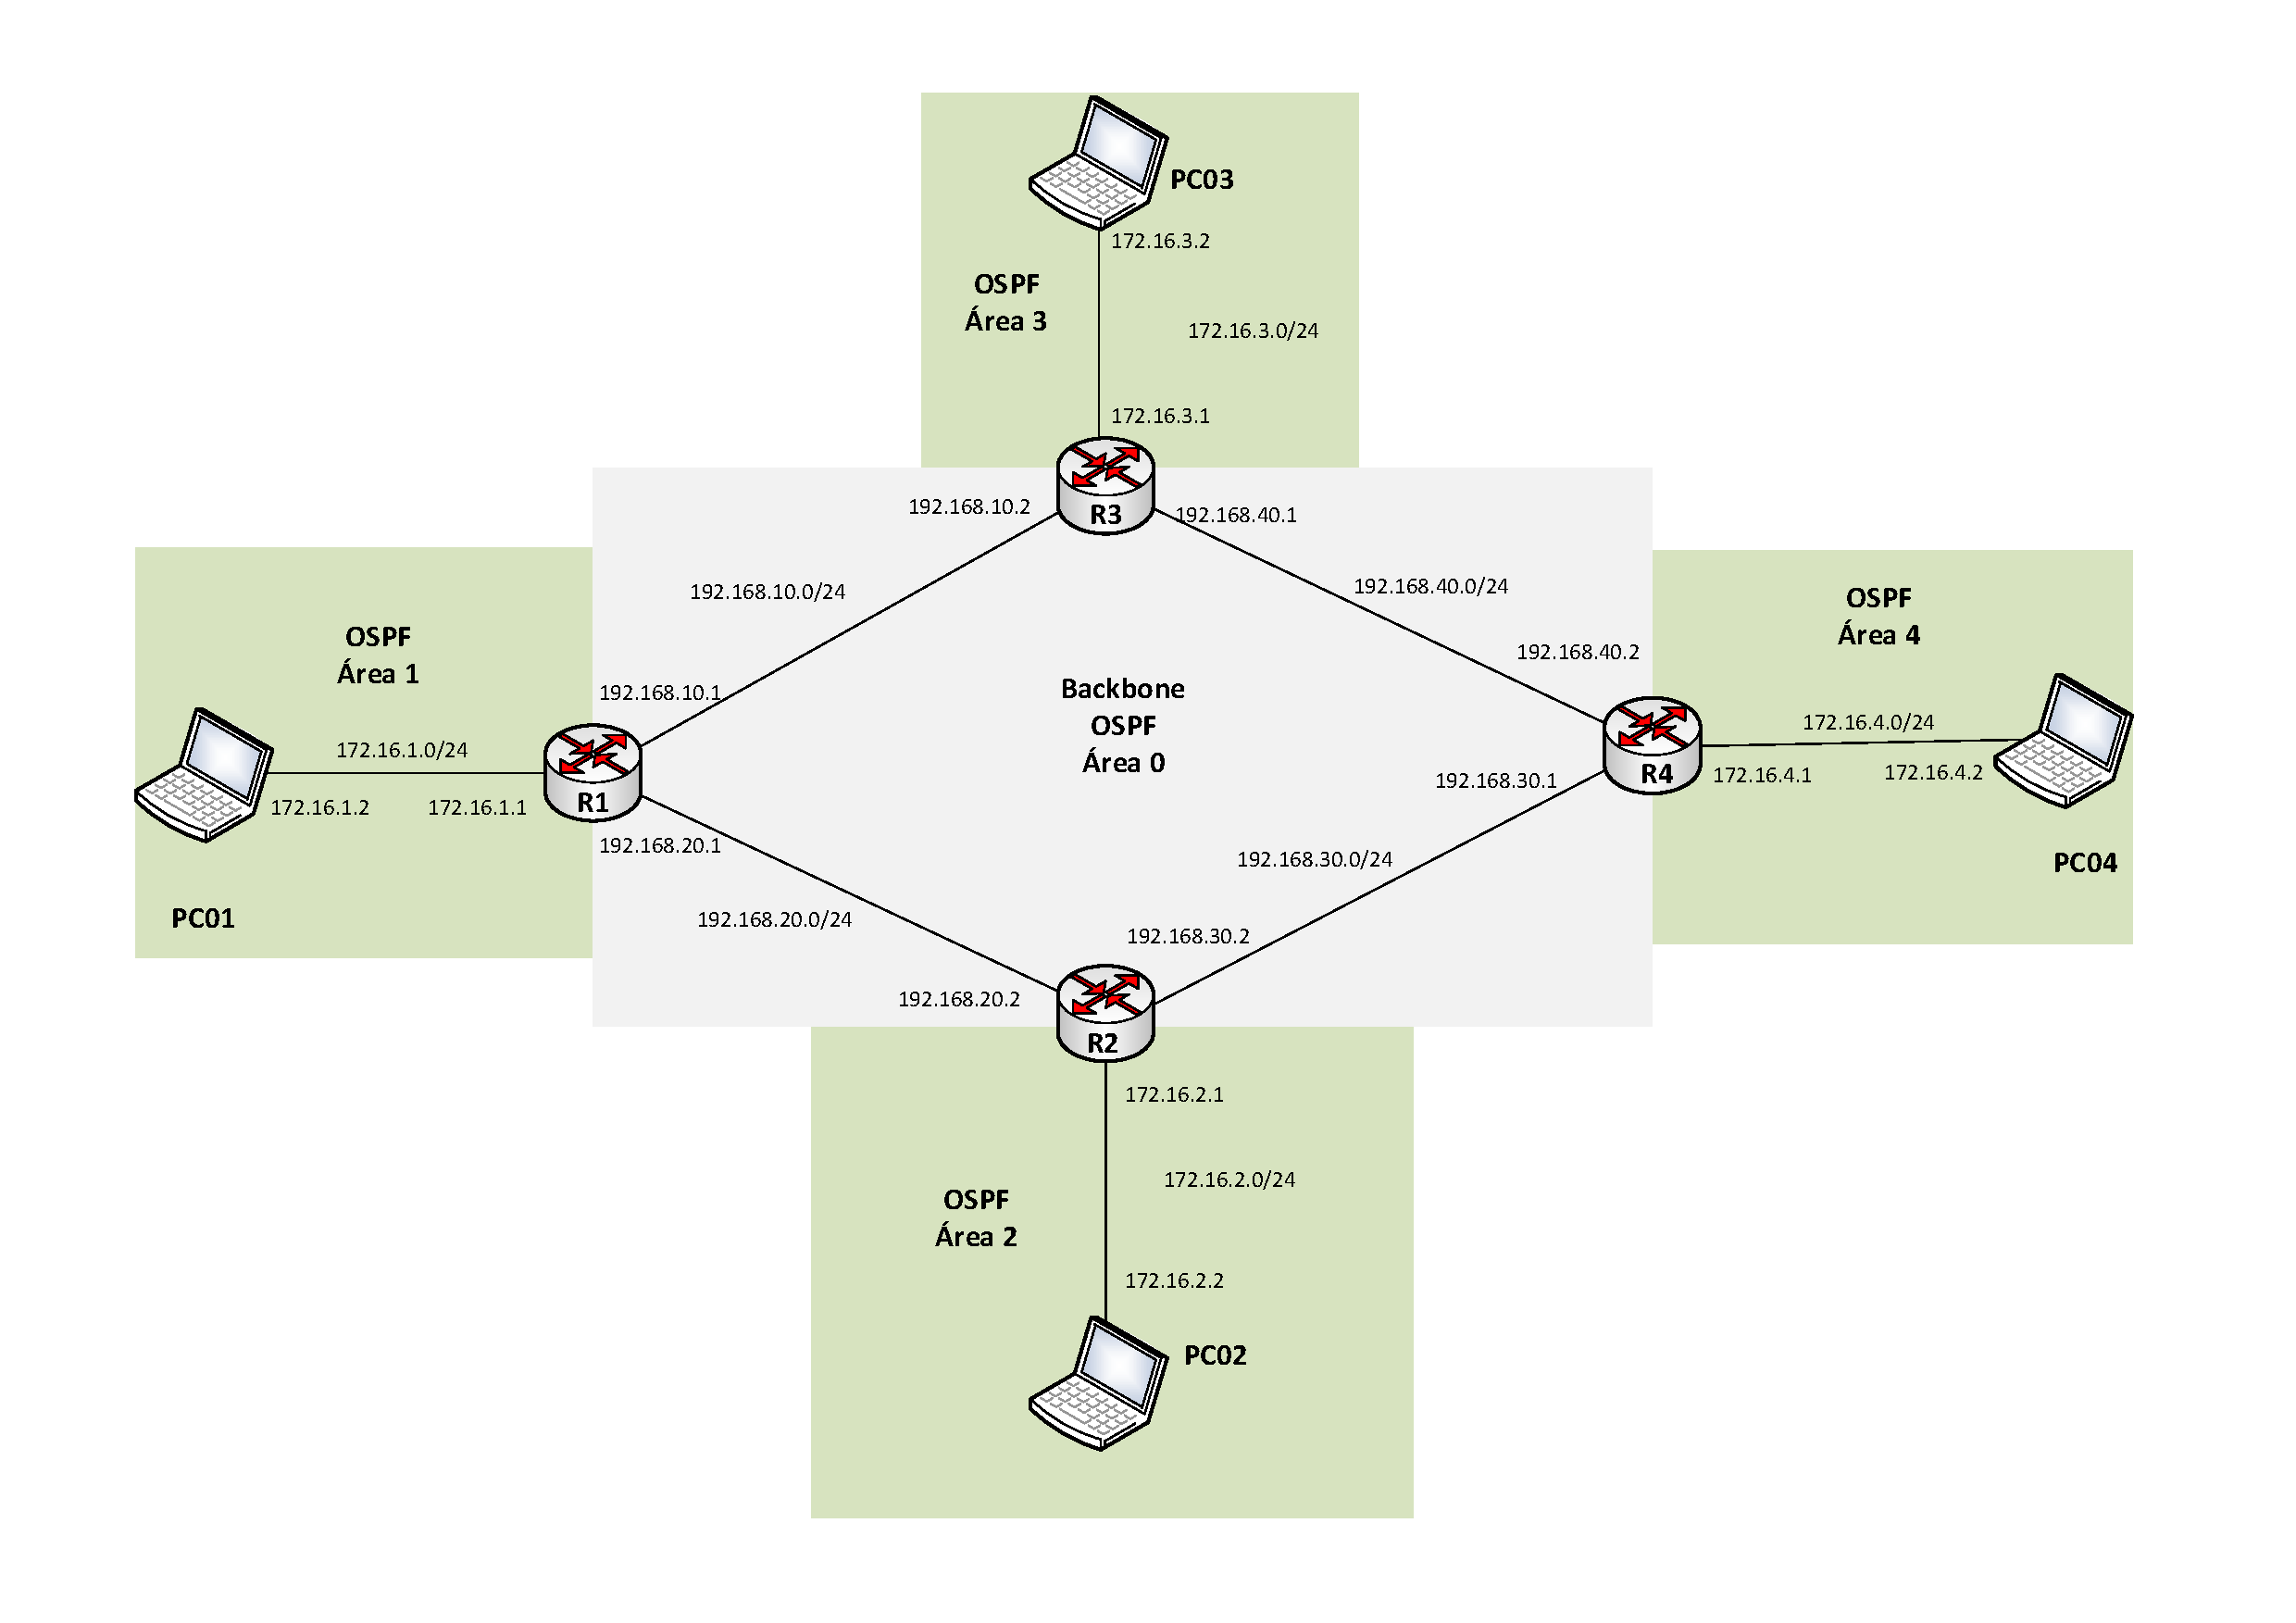
\includegraphics[width=\textwidth]{figs/topologia-2.pdf}
	\caption{Wired Network topology}
	\label{Fig01}
\end{figure*}

The remainder of this paper is organized to present the components and the architecture of a wired network based on context-aware routing. In Section II, the traditional routing protocols are revisited. In Section III, the proposed system and the environment parameters that may modify the routing context are presented. Section IV describes the results on the context-aware routing implementation for a wireless mesh network. Finally, in Section V, conclusions remarks are drawn. 